% -*- coding: UTF-8 -*-
% vim: autoindent expandtab tabstop=4 sw=4 sts=4 filetype=tex
% chktex-file 27 - disable warning about missing include files

\section{Beleuchtungsmodelle}
\label{sec:illumination_models}

Sofern im Text nicht anders vermerkt, basiert der folgende Abschnitt
auf~\cite[S. 343]{whitted_improved_1980}, sowie
auf~\cite{hughes_computer_2013}.

Beleuchtungsmodelle beschreiben, wieviel Licht von einem sichtbaren
Punkt einer Oberfläche zum Betrachter emittiert wird. In der Regel wird
das Licht als Funktion in Abhängigkeit folgender Faktoren beschrieben:

\begin{itemize}
    \item Richtung der Lichtquelle
    \item Lichtstärke
    \item Position des Betrachters
    \item Orientierung der Oberfläche
    \item Oberflächenbeschaffenheit
    \item Globale Umgebung
\end{itemize}

Dabei wird zwischen lokalen und globalen Belechtungsmodellen
unterschieden.

\subsection{Lokale Beleuchtungsmodelle}
\label{subsec:local_illumination_models}

Lokale Beleuchtungsmodelle aggregieren Daten lokal, also von
benachbarten Oberflächen. Diese Modelle sind in ihrem Umfang allerdings
limitiert, da sie normalerweise nur Lichtquellen sowie die Orientierung
einer Oberfläche einbeziehen. Sie ignorieren dabei aber die globale
Umgebung, in welcher sich eine Oberfläche befindet.  Die traditionell
verwendeten Algorithmen zur Berechnung der Sichtbarkeit von Oberflächen
verfügen über keine globalen Daten.\\
Das bekannteste lokale Beleuchtungsmodell ist das
\textit{Phong-Beleuchtungsmodell}, welches 1975 von Phong Bui-Tong
entwickelt wurde\parencite{phong_illumination_1975}. Es beschreibt
nicht-perfekte Reflektoren wie sie zum Beispiel ein
Apfel darstellt~\parencite[Kapitel 16, Seite 729]{foley_computer_1996}.

\begin{figure}[H]
    \centering
    
\includegraphics[width=0.6\textwidth]{img/phong_illumination_model.pdf}
    \caption{Illustration des Phong-Beleuchtungsmodelles\protect\footnotemark}\label{fig:phong_illustration}
\end{figure}
\footnotetext{Eigene Darstellung mittels Geogebra, angelehnt an~\cite{foley_computer_1996}[Kapitel 16, Seite 731, Abbildung 16.12]}

Das \textit{Phong-Beleuchtungsmodell} beschreibt die reflektierte
(Licht-) Intensität $I$ als Zusammensetzung aus der ambienten, der
diffusen und der ideal spiegelnden Reflexion einer Oberfläche:

\begin{gather}
    I = I_{\text{ambient}} + I_{\text{diffuse}} + I_{\text{specular}} + I_{\text{emissive}}
\end{gather}

Oder mathematisch ausgedrückt:

\begin{gather}\label{eq:phong_equation}
    I(\vv{V}) = k_{a} \cdot L_{a} +
                k_{d} \displaystyle\sum_{i=0}^{n - 1} L_{i} \cdot (\vv{S_{i}} \cdot \vv{N}) +
                k_{s} \displaystyle\sum_{i=0}^{n - 1} L_{i} \cdot {(\vv{R_{i}} \cdot \vv{V})}^{k_{e}}
\end{gather}

In der obigen Gleichung~\ref{eq:phong_equation} wurde der emissive Term
$I_{\text{emissive}}$ bewusst weggelassen, da er meistens für
Spezialeffekte statt für die Beleuchtung ``normaler'' Objekte benutzt
wird~\parencite{hughes_computer_2013}.

Wobei gilt:

\begin{itemize}
    \item $I(\vv{V})$\\
        Die reflektierte (Licht-) Intensität in Richtung des Vektors
        $\vv{V}$.

    \item $n$\\
        Anzahl Lichtquellen.

    \item $k_{a} \cdot L_{a}$\\
        Ambiente Komponente des Beleuchtungsmodelles. Mittels diesem
        Faktor wird versucht allem indirekten Licht der Szene gerecht zu
        werden. Bei $k_{a}$ handelt es sich um eine Konstante, welche
        den ambienten Anteils des Lichtes $L_{a}$ skaliert.

    \item $k_{d}$\\
        Konstante für die diffuse Komponente des reflektierten Lichtes,
        basierend auf der Wellenlänge bzw.\ der Frequenz.

    \item $\vv{S_{i}}$\\
        Richtung, in welcher das Licht der $i$-ten Lichtquelle ankommt,
        normalisierter Einheitsvektor.

    \item $\vv{N}$\\
        Einheitsnormale der Oberfläche.

    \item $k_{s}$\\
        Koeffizient der spiegelnden Komponente, basierend auf der
        Wellenlänge bzw. Frequenz.

    \item $\vv{R_{i}} = \vv{S_{i}} + 2(\vv{S_{i}} \cdot \vv{N})\vv{N}$\\
        Richtung, in welche das Licht der $i$-ten Lichtquelle
        reflektiert wird, normalisierter Einheitsvektor.

    \item $\vv{V}$\\
        Blickrichtung des Betrachters bzw.\ der Kamera.

    \item $k_{e}$\\
        Exponent, welcher von der Rauheit
        bzw.  Reflexion der Oberfläche abhängt.
    \item $L_{i}$\\
        Licht- bzw.\ Farbenintensität der $i$-ten Lichtquelle.
\end{itemize}

Der reflektive Vektor $\vv{R_{i}}$ ist gegeben durch

\begin{gather}
    \vv{R_{i}} = \vv{S_{i}} + 2(\vv{S_{i}} \cdot \vv{N})\vv{N}
\end{gather}

Damit die Energieerhaltung gewährleistet ist, muss weiter $k_{d} + k_{s}
< 1$ gelten. Der Winkel zwischen $\vv{R}$ und $\vv{V}$ wird mittels
$\cos(\alpha)$ ermittelt.

% -*- coding: UTF-8 -*-
% vim: autoindent expandtab tabstop=4 sw=4 sts=4 filetype=tex
% vim: spelllang=de spell
% chktex-file 27 - disable warning about missing include files

\subsection{Globale Beleuchtungsmodelle}
\label{subsec:global_illumination_models}

Sofern im Text nicht anders vermerkt, basiert der folgende Abschnitt
auf~\cite[S. 775ff]{foley_computer_1996}.

Globale Beleuchtungsmodelle beschreiben die (Licht-) Intensität eines
Punktes. Die Intensität setzt sich aus direkter und indirekter
Einstrahlung des Lichtes zusammen.

Direktes Licht kommt unbeeinflusst aus einer Lichtquelle direkt zum
Betrachter bzw.~zu einem Bildpunkt. Indirektes Licht entsteht durch
Diffusion, Reflexion und Transmission, je nach Beschaffenheit der Körper
sowie deren Oberfläche.

Bei globalen Beleuchtungsmodellen unterscheidet man zwischen Blickwinkel
abhängigen, z.B.~Ray Tracing, und zwischen Blickwinkel
unabhängigen Algorithmen, z.B.~Photon Mapping.

Blickwinkel abhängige Algorithmen verwenden eine Diskretisierung der
sichtbaren Fläche bzw.\ Bildfläche (Zerlegung in kleine Abschnitte, also
Bildpunkte). Dadurch kann entscheiden werden, von welchen Punkten, in
Blickrichtung des Betrachters gesehen, die Berechnung der Beleuchtung
durchgeführt werden soll.

Blickwinkel unabhängige Algorithmen hingegen diskretisieren die
Umgebung. Sie stellen so genügend Informationen zur Verfügung, um die
Berechnung der Beleuchtung an einem beliebigen Punkt unabhängig von der
Blickrichtung des Betrachters zu berechnen.

Beide Arten von Algorithmen haben Vor- und Nachteile.  Blickwinkel
abhängige Algorithmen eignen sich gut für die Berechnung von
Spiegelungen, welche auf der Blickrichtung des Betrachters basieren.
Sie eignen sich aber weniger um gleichbleibende diffuse Anteile über
weite Flächen eines Bildes zu berechnen.\\
Bei Blickwinkel abhängigen Algorithmen ist genau das Gegenteil der Fall.

\subsubsection{Renderinggleichung}
\label{ssubsec:rendering_equation}

Die unter~\ref{subsec:global_illumination_models} genannten Verfahren
berechnen, wie sich Licht von einem Punkt $A$ zu einem anderen Punkt $B$
im Raum bewegt. Dabei beschreiben sie die Intensität des Lichtes von $A$
nach $B$. Zusätzlich werden alle Intensitäten von beliebigen Punkten im
Raum, die den Punkt $A$ erreichen und zu Punkt $B$ reflektiert werden,
mit einberechnet.

James Kajiya stellte 1986 die so genannte Renderinggleichung auf, welche
dieses Verhalten
beschreibt~\parencites{kajiya_rendering_1986}{foley_computer_1996}:

\begin{equation}
    I(x, x') = g(x, x')[\varepsilon(x, x') + \int\limits_{S}\rho(x, x', x'')I(x', x'')dx'']
\end{equation}

Wobei gilt:

\begin{itemize}
    \item $x, x' \text{und } x''$\\
        Punkte im Raum.
    \item $ I(x, x')$\\
        Intensität des Lichtes, die von Punkt $x'$ zu Punkt $x$ gelangt.
    \item $ g(x, x')$\\
        Ein auf die Geometrie bezogener Term\\
        \hspace*{4mm} $0$:     \hspace*{6mm} $x$ und $x'$ verdecken
                               sich.\\
        \hspace*{4mm} $1/r^2$: \hspace*{1mm} $x$ und $x'$ sehen sich,
                               wobei $r$ die Distanz zwischen $x$ und
                               $x'$ ist.
    \item $\varepsilon(x, x')$\\
        Intensität des Lichtes, welches von $x'$ nach $x$ emittiert
        wird.
    \item $\rho(x, x', x'')$\\
        Intensität des Lichtes, welches von $x''$
        durch die Oberfläche bei $x'$ nach $x$
        gestreut wird.
    \item $\int\limits_{S}$\\
        Integral über die Vereinigung aller Flächen, daher $ S =
        \bigcup{S_{i}} $.\\ Dies bedeutet, dass die Punkte $x$, $x'$ und
        $x''$ über alle Flächen aller Objekte der Szene ``streifen''.
        Wobei es sich bei $S_{0}$ um eine zusätzliche Fläche handelt,
        welche als Hintergrund verwendet wird.  $S_{0}$ ist dabei eine
        Hemisphäre, welche die gesamte Szene umspannt.
\end{itemize}

\section{Ray Casting und Ray Tracing}
\label{sec:ray_casting_tracing}

Sofern nicht anders vermerkt, basiert der folgende Abschnitt
auf~\cite[Kapitel 15, S. 387ff]{hughes_computer_2013}.

Um ein Bild möglichst realistisch darzustellen muss berechnet werden, wieviel
Licht zu jedem Pixel der sichtbaren Bildfläche (also dem Betrachter)
transportiert wird. Da Photonen die Energie des Lichtes transportieren,
möchte man das physikalische Verhalten dieser simulieren.

Es ist allerdings nicht möglich \textit{alle} Photonen zu simulieren, da
der Aufwand schlicht zu gross wäre. Daher macht es Sinn nur einige
Photonen (exemplarisch) zu betrachten und dann eine Abschätzung des
gesamten Lichtes vorzunehmen.

Jede Lichtquelle emittiert Photonen (als Welle und als Teilchen) in alle
Richtungen. Man modelliert diese als Partikel, welche anhand
Lichtstrahlen (\textit{light rays}) auf Objekte einer
Szene treffen.

Jedes Photon hat dabei eine spezifische Wellenlänge $\lambda{}$, welche
die Farbe definiert, sowie eine Energie respektive Frequenz $f$, welche
die Intensität der Farbe des Photons definiert.

Trifft ein Photon auf ein Objekt, wird ein Teil der Energie absorbiert,
ein Teil reflektiert und ein Teil durchdringt das Objekt (Transmission).
Photonen treffen solange auf Objekte, bis deren gesamte Energie
absorbiert, sie die Szene verlassen oder sie auf die sichtbare
Bildfläche treffen und somit zum eigentlichen Bild beitragen.

Bei \textit{Ray Casting} bzw. \textit{Ray Tracing} handelt es sich um
zwei relativ einfache Verfahren um globale Beleuchtungsmodelle zu
implementieren.

Die einfachste Art das oben genannte Verhalten von Licht zu modellieren
ist das so genannte~\textit{Ray Casting}.

% -*- coding: UTF-8 -*-
% vim: autoindent expandtab tabstop=4 sw=4 sts=4 filetype=tex
% vim: tw=72
% vim: spelllang=de spell
% chktex-file 27 - disable warning about missing include files

\subsection{Ray Casting}
\label{subsec:ray_casting}

\textit{Ray Casting} ist ein Verfahren zur Simulation, wieviel Licht
anhand eines (Licht-) Strahles zu der sichtbaren Bildfläche (also dem
Betrachter) transportiert wird.

Das Verfahren wurde erstmals
in~\citetitle{appel_techniques_1968}~\citeyear{appel_techniques_1968}
von~\citeauthor{appel_techniques_1968} vorgeschlagen und
auch~\citeyear{arlington_mathematical_applications_group_inc_afips_1968}
von
der~\citeauthor{arlington_mathematical_applications_group_inc_afips_1968}
in~\citetitle{arlington_mathematical_applications_group_inc_afips_1968}
erfolgreich umgesetzt.

Ein möglicher Algorithmus, wie Ray Casting umgesetzt werden kann, findet
sich in~\autoref{fig:ray_casting:high_level}.

Bei dem Ray Casting Verfahren wird ein \textit{Projektionszentrum} (das
Auge eines Betrachters) sowie eine Region einer beliebigen Bildfläche
gewählt. Dabei kann die Region als gerasterte Fläche angenommen werden.
Jedes Raster entspricht den Bildpunkten (Pixeln) der gewünschten
Auflösung. Je feiner die Rasterung, desto höher die Auflösung.

Für jeden Bildpunkt der gewählten Region wird ein Strahl generiert,
welcher dann vom Projektionszentrum durch das Zentrum des Bildpunktes
auf die Szene ``geworfen'' wird. 

Es wird dann das Objekt gesucht, welches den nächsten Schnittpunkt mit
dem Strahl bildet. Für jede Lichtquelle der Szene wird geprüft, ob die
Lichtquelle vom Schnittpunkt aus sichtbar ist. Ist dies der Fall, wird
schliesslich die Farbe und die Intensität der Farbe an diesem Schnittpunkt
anhand eines Beleuchtungsmodelles (z.B.\ dem Phong-Beleuchtungsmodell)
berechnet. Andernfalls befindet sich der Punkt im Schatten, er wird also
nicht beleuchtet.

\begin{figure}[H]
    \centering
    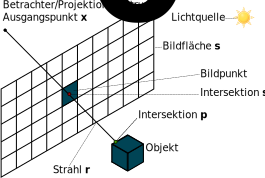
\includegraphics{img/ray_casting.pdf}
    \caption{Illustration des Ray Casting Verfahrens\protect\footnotemark}\label{fig:ray_casting_illustration}
\end{figure}
\footnotetext{Eigene Darstellung mittels Inkscape}

Die obenstehende~\autoref{fig:ray_casting_illustration} zeigt das
Prinzip des Ray Castings. Ausgangspunkt bildet der Betrachter mit $x_{0}
= (x_{x_{0}}, y_{x_{0}}, z_{x_{0}})$. Es wird ein Strahl $r = (x_{0},
d)$ in Richtung $d$ der Bildfläche $s$ ``geworfen''. Der Strahl $r$
schneidet die Bildfläche $s$ an einem Punkt $sp = (x_{sp}, y_{sp},
z_{sp})$.  Somit ergibt sich die Richtung des Strahles $d = sp - x_{0} =
(x_{sp} - x_{x_{0}}, y_{sp} - y_{x_{0}}, z_{sp} - z_{x_{0}}) = (x_{d},
y_{d}, z_{d})$. Der Strahl $r$ trifft und schneidet schliesslich ein
Objekt am Punkt $p = r(t) = x_{0} + t \cdot d$ wobei $t \in [1, \infty]$
ist. Dies führt dazu, dass dem Raster respektive dem Bildpunkt, durch
welchen der Strahl $r$ hindurch geht, die Farbe des getroffenen Objektes
zugewiesen wird.

\subsubsection{Berechnung von Schnittpunkten}
\label{ssubsec:ray_casting_intersections}

Um den Schnittpunkt eines Lichtstrahles mit einem Objekt zu berechnen,
wird grundsätzlich die mathematische Gleichung des Lichtstrahles in die
des Objektes eingesetzt. Existiert eine reelle Lösung, so schneidet der
Lichtstrahl das Objekt am nächsten Punkt zwischen dem Schnittpunkt und
der Oberflächennormale des Objektes.

~\citeauthor{glassner_introduction_1989} beschreibt mehrere Methoden zur
Prüfung von Schnittpunkten: Beispielsweise seien hier die Intersektionen
eines Strahles mit einer Kugel oder mit einem Dreieck gezeigt.

\textit{Schnittpunkt mit einer Kugel}

Um den Schnittpunkt bzw.\ die Schnittpunkte eines Lichtstrahles mit
einer Kugel zu erhalten, wird die Gleichung des Lichtstrahles

\begin{gather}\label{eq:ray_equation}
    r(t) = r_{0} + t \cdot r_{d}
\end{gather}

in die implizite Gleichung einer Kugel

\begin{gather}
    \|\bm{x} - c\|^{2} - r^{2} = 0
\end{gather}

eingesetzt. Dies führt zu folgender Gleichung zweiten Grades:

\begin{align}
    \|r(t) - c\|^{2} - r^{2} &= 0 \\
    \|r_{0} + t \cdot r_{d} - c\|^{2} - r^{2} &= 0
\end{align}

Das Auflösen dieser Gleichung ergibt folgende Fälle:

\begin{itemize}
    \item{Zwei Lösungen}: Der Strahl geht durch die Kugel hindurch.
    \item{Eine Lösung}: Der Strahl streift die Kugel an einem Punkt als
        Tangente.
    \item{Imaginäre Lösung}: Der Strahl verfehlt die Kugel.
\end{itemize}


\textit{Schnittpunkt mit einem Dreieck}

Um den Schnittpunkt eines Lichtstrahles mit einem Dreieck zu erhalten,
wird die~\autoref{eq:ray_equation} des Lichtstrahles als Lösung
der Gleichung eines Dreiecks mit baryzentrischen Koordinaten

\begin{gather}
    x(\beta, \gamma) = v_{1} + \beta(v_{2} - v_{1}) + \gamma(v_{3} - v_{1})
\end{gather}

verwendet. Dies führt zu folgendem Gleichungssystem:

\begin{align}
    r_{0} + t \cdot r_{d} &= v_{1} + \beta(v_{2} - v_{1}) + \gamma(v_{3} - v_{1})
\end{align}

Der Lichtstrahl schneidet das Dreieck, wenn die Summe der Koeffizienten
($\beta$, $\gamma$) $\le 1$ ist.

Es leuchtet ein, dass es sehr aufwändig ist jegliches Objekt einer Szene
auf Schnittpunkte zu testen (wie dies in
~\autoref{fig:ray_casting:high_level} getan wird). Um das Auffinden von
Schnittpunkten zu beschleunigen, möchte man den durchschnittlichen
Aufwand reduzieren. Dies kann geschehen durch effizientere Algorithmen,
z.B.~durch Verwendung von Hüllköpern, oder durch Reduktion der
Schnittstellen, z.B. durch Verwendung von Hierarchien von Hüllkörpern
oder der Unterteilung des Raumes einer Szene.

Einen guten Überblick bietet das Kapitel ``A Survey of Ray Tracing
Accelelration Techiques'' in~\citetitle[S.
202ff]{glassner_introduction_1989},
von~\cite{glassner_introduction_1989}.

\begin{minipage}{\linewidth}
\begin{lstlisting}[language=Python,caption={Eine abstrakte Umsetzung des Ray
        Casting
Verfahrens\protect\footnotemark.},label={fig:ray_casting:high_level},captionpos=b,emph={ray_cast}]
def ray_cast():
    # "pixels" is a list of all pixels of the image plane
    for pixel in pixels:
        # Save all intersections for given pixel
        intersections = []

        # Returns the ray passing through the given
        # pixel from the eye
        ray = ray_at_pixel(pixel)

        # "scene_triangles" is a list of all triangles
        # coming from meshes contained in the scene to render
        for triangle in scene_triangles:
            p   = intersect(ray, triangle)
            sum = 0

            for light in incoming_lights_at_p:
                sum = sum + l.value
            end

            if is_smallest_intersection(p, intersections):
                pixel = sum
            intersections.append(p)
\end{lstlisting}
\end{minipage}
\footnotetext{Algorithmus in Pseudocode gemäss~\cite[Kapitel 15, Seite 391, Auflistung 15.2]{hughes_computer_2013}}

% -*- coding: UTF-8 -*-
% vim: autoindent expandtab tabstop=4 sw=4 sts=4 filetype=tex
% vim: tw=72
% vim: spelllang=de spell
% chktex-file 27 - disable warning about missing include files

\subsection{Ray Tracing}
\label{subsec:ray_tracing}

Sofern im Text nicht anders vermerkt, basiert der folgende Abschnitt
auf~\cite[S. 1 bis 77]{glassner_introduction_1989}.

Bei dem heute als Ray Tracing bekannten Verfahren handelt es sich um
eine verbesserte Version des unter~\ref{subsec:ray_casting} genannten
Ray Casting Verfahrens. \citeauthor{whitted_improved_1980} publizierte
das Verfahren~\citeyear{whitted_improved_1980} im
Paper~\citetitle{whitted_improved_1980}.

Ein möglicher Algorithmus, wie Ray Tracing umgesetzt werden kann, findet
sich in~\autoref{fig:ray_tracing:high_level}.

Analog dem Ray Casting Verfahren wird wieder ein Projektionszentrum (das
Auge eines Betrachters) sowie eine Region einer beliebigen Bildfläche
gewählt.

Jeder Bildpunkt der gewählten Region erhält Licht aus nur einer Richtung
--- der Richtung der Lichtstrahlen (\textit{light rays}), welche durch
die gewählte Region und die sichtbare Bildfläche gehen. Somit trägt
jedes Photon, welches aus dieser Richtung kommt, zum Farbwert bzw.\ der
Intensität der Farbe eines Bildpunktes bei. Strahlen, welche das Licht
direkt zur sichtbaren Bildfläche transportieren, werden \textit{Pixel}-
bzw.\ \textit{Augen-Strahlen} genannt~\parencite[S.
10]{glassner_introduction_1989}.

\begin{figure}[H]
    \centering
    \includegraphics{img/ray_tracing_scene.pdf}
    \caption{Illustration des Prinzips des Ray Tracing
        Verfahrens\protect\footnotemark}\label{fig:ray_tracing_scene}
\end{figure}
\footnotetext{Eigene Darstellung mittels Inkscape angelehnt
    an~\cite{glassner_introduction_1989}[S. 16]}

Die Strahlen werden vom Betrachter aus verfolgt, um festzustellen wie
das Licht ``erzeugt'' wird. Trifft der Strahl ins Leere, wird seine
Verfolgung beendet und der entsprechende Bildpunkt wird mit der Farbe
des Hintergrundes eingefärbt. Trifft der Strahl direkt auf eine
Lichtquelle wird seine Verfolgung beendet und der Bildpunkt wird mit der
Farbe und Intensität der Lichtquelle eingefärbt. Trifft der Lichtstrahl
auf eine Oberfläche, wird der Prozess der Strahlenverfolgung von diesem
Punkt aus neu gestartet um festzustellen, wie die Beleuchtung dort zu
Stande kam.

Wie der letzte Punkt zeigt, handelt es sich um ein rekursives Verfahren
und wird daher zum Teil auch rekursives Ray Tracing genannt. Im
Unterschied zu Ray Tracing kennt Ray Casting keine Rekursion.

Zur Berechnung des emittierten Lichtes an einem bestimmten Punkt auf der
Oberfläche eines Objektes, wird in einem ersten Schritt die Intensität
des Lichtes dieses Punktes bestimmt. Man spricht dabei von
\textit{Licht}- bzw.\ \textit{Schatten-Strahlen}~\parencite[S.
10]{glassner_introduction_1989}.

In einem weiteren Schritt wird berechnet, wie die Oberfläche an
diesem Punkt Licht in eine spezifische Richtung weiterleitet, basierend
auf der physikalischen Beschaffenheit der Oberfläche.

Trifft ein Lichtstrahl auf eine Oberfläche, wird dieser zu gewissen
Teilen~\textit{absorbiert}, \textit{reflektiert} und \textit{gebrochen}.
Die jeweiligen Anteile hängen dabei vom Medium der Oberfläche bzw.~des
Objektes, der Frequenz des Lichtes sowie zwischen dem eingehenden Winkel
des Lichtstrahles und der Oberflächennormale ab.  Licht kann je nach
Medium auch gestreut werden.

Für den Transport des Lichtes kennt man vier Mechanismen: Perfekt
diffuse, perfekt spiegelnde und totale interne Reflexion sowie perfekt
brechende Refraktion~\parencite[S. 130 bis
137]{glassner_introduction_1989}. In der Realität bzw.~der Natur treten
mehrere Mechanismen gleichzeitig auf.  So wird z.B.\ ein Teil des
Lichtes reflektiert, wohingegen ein anderer Teil das Objekt durchdringt.

Die von diesen Mechanismen emittierten Strahlen können
gemäss~\citeauthor{glassner_introduction_1989}
in~\textit{Reflexion-Strahlen}, welche die perfekte diffuse und die
perfekt spiegelnde Reflexion beschreiben,
und~\textit{Transparenz-Strahlen}, welche die perfekt brechende
Refraktion und die totale interne Reflexion beschreiben, unterteilt
werden~\parencite[S.  10]{glassner_introduction_1989}.

\begin{figure}[H]\label{fig:ray_tracing_scene_rays}
    \centering
    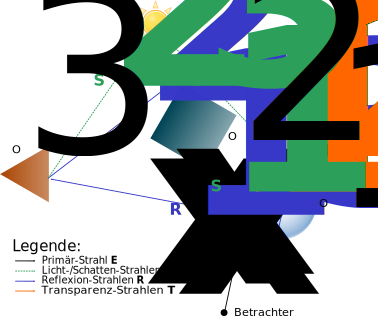
\includegraphics{img/ray_tracing_scene_rays.pdf}
    \caption{Illustration der einzelnen Strahlen und deren Verhalten
        ausgehend von der Szene in
        \autoref{fig:ray_tracing_scene}.\protect\footnotemark{} Das im
        Bild ersichtliche, orange-farbige Dreieck hat eine
        undurchlässige, reflexive Oberfläche. Der türkis-farbige Würfel
        hat eine diffuse Oberfläche.  Bei der Kugel, rechts im Bild,
        handelt es sich um eine Kugel aus Glas, welche das Licht
        teilweise bricht und reflektiert.}
\end{figure}

\footnotetext{Eigene Darstellung mittels Inkscape angelehnt
    an~\cite[S. 16]{glassner_introduction_1989}}

Nachfolgend werden die oben genannten Strahlen im Einzelnen beschrieben.

\subsubsection{Augen- oder Pixel-Strahlen}
\label{ssubsec:ray_tracing:eye_rays}

Augen- oder Pixel-Strahlen sind Strahlen, welche das Licht von einer
Lichtquelle durch einen Bildpunkt direkt zu der sichtbaren Bildfläche
(also dem Betrachter) transportieren.

Die Gleichung solcher Strahlen lautet:

\begin{gather}
    r(t) = x_{0} + t \cdot (S - x_{0})
\end{gather}

Dabei ist $x_{0}$ der Ausgangspunkt (also der Betrachter), $t$ ein
Skalierungsfaktor zwischen $[1, \infty]$ und $S$ der Schnittpunkt mit der
Bildfläche.

\subsubsection{Licht- oder Schatten-Strahlen}
\label{ssubsec:ray_tracing:shadow_rays}

Bei Licht- bzw.\ Schatten-Strahlen handelt es sich um Strahlen, welche
das Licht von einer Lichtquelle direkt zu der Oberfläche eines Objektes
transportieren. Bei jedem Schnittpunkt eines Primär-Strahles (ein Strahl
welcher vom Betrachter aus in die Szene ``geworfen'' wird) mit einem
Objekt wird ein Schatten- bzw.\ Licht-Strahl in Richtung jeder
Lichtquelle der Szene ``geworfen''. Trifft der Schatten- bzw.\
Licht-Strahl die Lichtquelle, wird das Licht zur Berechnung der Farbe
und Intensität des Lichtes genutzt. Trifft der Schatten-Strahl keine
Lichtquelle, so wird das Licht nicht berücksichtigt. Schatten-Strahlen
generieren keine weiteren Strahlen.

Die Gleichung von Licht- bzw.\ Schatten-Strahlen lautet:

\begin{gather}
    r(t) = p_{0} + t \cdot (L_{i} - p_{0})
\end{gather}

Dabei ist $p_{0}$ der Ausgangspunkt (also ein Punkt auf einer Oberfläche
eines Objektes), $t$ ein Skalierungsfaktor zwischen $[\varepsilon, 1]$ und
$L_{i}$ der Ort der $i$-ten Lichtquelle. Bei $\varepsilon$ handelt es
sich um einen Faktor zur Steuerung der Präzision, welcher verhindert,
dass ein Objekt lokal auf sich selbst Schatten wirft.

\subsubsection{Reflexion-Strahlen}
\label{ssubsec:ray_tracing:reflection_rays}

Das Verhalten von (Licht-) Strahlen, welche auf ein Objekt treffen und
an diesem gespiegelt werden, wird durch~\textit{Reflexion-Strahlen}
beschrieben. Wie oben beschrieben, unterscheidet man zwei Arten der
Reflexion: Perfekt diffuse und perfekt spiegelnde Reflexion.

\textbf{Perfekt spiegelnde Reflexion}

Bei der perfekt spiegelnden Reflexion verlässt der ausgehende Strahl die
Oberfläche im selben Winkel wie der einfallende Strahl. Der
Ausfallswinkel entspricht also dem Einfallswinkel.

Die Gleichung eines Strahles, welcher von einer perfekt spiegelnden
Reflexion ausgeht, lautet~\parencite[S. 132]{glassner_introduction_1989}:

\begin{align}
    r(t) &= p_{0} + t \cdot R \\
    R &= I - 2(I \cdot N)N
\end{align}

Dabei sind $p_{0}$ der Ausgangspunkt (also ein Punkt auf einer Oberfläche
eines Objektes), $t$ ein Skalierungsfaktor zwischen $[\varepsilon, 1]$, $I$
der eingehende Vektor, also $S - x_{0}$, und $N$ die Oberflächennormale.
Bei Epsilon handelt es sich wiederum um einen Faktor zur Steuerung
der Präzision. Er verhindert, dass ein Objekt lokal in sich selbst
gespiegelt wird.

\begin{figure}[H]\label{fig:ray_tracing_specular_reflection}
    \centering
    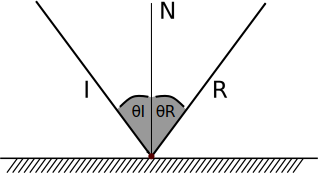
\includegraphics{img/perfect_specular_reflection.pdf}
    \caption{Illustration einer perfekt spiegelnden
        Reflexion.~\protect\footnotemark{}
        $I$ ist der eingehende Strahl, welcher am Normalenvektor $N$ der
        schraffierten Oberfläche in Richtung $R$ reflektiert wird. Der
        Winkel des eingehenden Strahles $\theta_{I}$ ist gleichgross wie der
        Winkel des ausgehenden Strahles $\theta_{R}$.}
\end{figure}
\footnotetext{Eigene Darstellung mittels Inkscape angelehnt
    an~\cite[S. 131]{glassner_introduction_1989}}

\textbf{Perfekt diffuse Reflexion}

Bei der perfekt diffusen Reflexion wird das eingehende Licht mit
gleicher Amplitude (also Stärke) gleichmässig in alle Richtungen
gestreut. Die Amplitude ist dabei proportional zum Kosinus des
Einfallswinkels und der Oberflächennormale.

\begin{figure}[H]\label{fig:ray_tracing_diffuse_reflection}
    \centering
    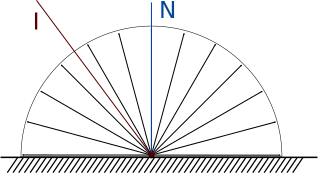
\includegraphics{img/perfect_diffuse_reflection.pdf}
    \caption{Illustration einer perfekt diffusen
        Reflexion.~\protect\footnotemark{}
        $I$ ist der eingehende Strahl, welcher am Ort des
        Normalenvektors $N$ der schraffierten Oberfläche auftrifft. Das
        Licht wird gleichmässig in alle Richtungen gestreut.}
\end{figure}
\footnotetext{Eigene Darstellung mittels Inkscape angelehnt
    an~\cite{glassner_introduction_1989}[S. 134]}

\subsubsection{Transparenz-Strahlen}
\label{ssubsec:ray_tracing:transparency_rays}

Schliesslich werden die Eigenschaften von Licht, welches durch ein
Objekt hindurch geht und vielleicht von diesem gebrochen wird, durch
die~\textit{Transparenz-Strahlen} beschrieben. Auch hier werden zwei
Arten der Reflexion unterschieden: Perfekt brechende Refraktion und
total interne Reflexion.

\textbf{Perfekt brechende Refraktion}

Tritt Licht von einem Medium (z.B.~Luft) in ein anderes Medium (z.B.\
Glas) ein, so wird das Licht abgelenkt. Die Ablenkung des Lichtes bei
Eintritt in ein neues Medium wird auch Transmission oder Refraktion
genannt. Dabei hat jedes Medium einen eignen Refraktions-Index
(Brechungsindex).\\
Der Refraktions-Index $n$ gibt das Verhältnis der
Vakuumlichtgeschwindigkeit $c_{0}$ zur Ausbreitungsgeschwindigkeit
$c_{M}$ des Lichtes in einem Medium $M$ an: $n = {c_{0} \over c_{M}}$.

Um zu berechnen, in welche Richtung das Licht abgelenkt wird, werden die
Refraktions-Indizes der Medien sowie der Einfalls- bzw. Ausfallswinkel
verglichen. Die Beziehung zwischen dem Einfalls- und Ausfallswinkel sowie dem
übertragenen Licht wird durch das Gesetz von ``Snell'' beschrieben:

\begin{gather}
    \frac{\sin(\theta_{1})}{\sin(\theta_{2})} = \eta_{21} = \frac{\eta_{2}}{\eta_{1}}
\end{gather}

Dabei ist $\theta_{1}$ der Einfallswinkel, $\theta_{2}$ der
Ausfallswinkel, $\eta_{1}$ der Refraktion-Index des ersten Mediums in
Abhängigkeit zu Vakuum, $\eta_{2}$ der Refraktion-Index des zweiten
Mediums in Abhängigkeit zu Vakuum und $\eta_{21}$ der Refraktion-Index
des zweiten Mediums in Abhängigkeit des ersten Mediums~\parencite[S. 134
bis 135]{glassner_introduction_1989}.

Umgekehrt kann das Verhältnis des ausgehenden Strahles zum eingehenden
Strahl berechnet werden~\parencite[S. 137 bis
140]{glassner_introduction_1989}:

\begin{gather}
    \eta_{12} = \frac{\eta_{1}}{\eta_{2}} = \frac{\sin(\theta_{2})}{\sin(\theta_{1})}
\end{gather}

Mithilfe dieses Verhältnisses kann der gebrochene Strahl berechnet
werden wie folgt~\parencite[S. 137 bis 140]{glassner_introduction_1989}:

\begin{align}
    r(t) &= p_{0} + t \cdot T \\
    T &= \eta_{12}I + (\eta_{12} \cdot C_{1} - \sqrt{C_{2}})N
    \label{eq:ray_tracing:transm} \\
    C_{1} &= -I \cdot N \\
    C_{2} &= 1 + \eta_{12}^{2}(C_{1}^{2} - 1) \label{eq:ray_tracing:transm_c2}
\end{align}

Dabei sind $p_{0}$ der Ausgangspunkt (also ein Punkt auf einer Oberfläche
eines Objektes), $t$ ein Skalierungsfaktor zwischen $[\varepsilon, 1]$, $I$
der eingehende Vektor, also $S - x_{0}$, $N$ die Oberflächennormale und
$\eta_{12}$ das oben beschriebene Verhältnis.
Bei Epsilon handelt es sich wie beschrieben um einen Faktor zur Steuerung
der Präzision. Er verhindert, dass ein Objekt lokal in sich selbst
gespiegelt wird.

\begin{figure}[H]\label{fig:ray_tracing_specular_transmission}
    \centering
    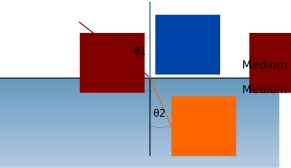
\includegraphics{img/perfect_specular_tranmission.pdf}
    \caption{Illustration einer perfekt brechenden
        Refraktion.~\protect\footnotemark{}
        $I$ ist der eingehende Strahl, welcher am Ort des
        Normalenvektors $N$ im Winkel von $\theta_{1}$ von Medium 1 in
        Medium 2 übergeht und entsprechend mit Winkel $\theta_{2}$
        anhand $T$ gebrochen wird.}
\end{figure}
\footnotetext{Eigene Darstellung mittels Inkscape angelehnt
    an~\cite[S.135]{glassner_introduction_1989}}

\textbf{Totale interne Reflexion}

Die totale interne Reflexion tritt dann auf, wenn Licht unter einem zu
flachen Winkel versucht von einem dichten Medium in ein weniger dichtes
Medium zu gelangen. Das Licht ``prallt'' am Übergang der beiden Medien ab
und wird gespiegelt anstatt in das andere Medium
einzutreten~\parencite[S. 136 bis 137]{glassner_introduction_1989}.

Dies geschieht nur dann, wenn der Term $C_{2}$
(siehe~\autoref{eq:ray_tracing:transm_c2}) negativ ist und somit das
Ergebnis der Wurzel aus $C_{2}$ in~\autoref{eq:ray_tracing:transm} eine
imaginäre Zahl wird~\parencite[S. 137 bis 138]{glassner_introduction_1989}.

\begin{figure}[H]\label{fig:ray_tracing_total_internal_reflection}
    \centering
    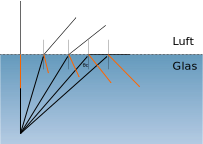
\includegraphics{img/total_internal_reflection.pdf}
    \caption{Illustration der totalen internen
        Reflexion.~\protect\footnotemark{}
        Ist der kritische Winkel $\theta_{c}$ beim Übertritt eines
        Strahles von einem Medium (hier Glas) zu einem anderen Medium (hier
        Luft) nicht überschritten, so wird der Strahl bzw.\ Licht sowohl
        gebrochen als auch reflektiert. Wird der kritische Winkel
        überschritten, so findet nur noch eine Reflexion
        statt.\protect\footnotemark}
\end{figure}
\addtocounter{footnote}{-2}
\stepcounter{footnote}\footnotetext{Eigene Darstellung mittels Inkscape angelehnt
    an~\cite[S. 137]{glassner_introduction_1989}}
\stepcounter{footnote}\footnotetext{\cite[S. 137]{glassner_introduction_1989}}

\subsubsection{Modelle zur Schattierung (shading models)}
\label{ssubsec:ray_tracing:shading_models}

\citeauthor{glassner_introduction_1989} beschreibt auf der Physik
basierende Modelle zur Schattierung (shading models), welche heute unter
dem Begriff PBRT --- Physically Based Rendering bekannt sind. Diese
hier aufzuführen würde den Rahmen dieser Projektarbeit sprengen. Daher
wird darauf verzichtet. Der interessierte Leser sei
auf~\citetitle[S. 143ff]{glassner_introduction_1989},
sowie~\citetitle{pharr_physically_2010} verwiesen.

\subsubsection{Rekursion und Strahlen-Baum}
\label{ssubsec:ray_tracing:recursion}

Sofern im Text nicht anders vermerkt, basiert der folgende Abschnitt
auf~\cite[S. 16 bis 17]{glassner_introduction_1989}.

Wie zu Beginn des Kapitels bereits angesprochen wurde, handelt es sich
bei Ray Tracing um ein rekursives Verfahren. Es stellt sich somit die
Frage, wie tief die Rekursion gehen soll und auch kann.\\
Zusätzlich zu dem genannten Fall, dass ein Strahl auf kein Objekt
innerhalb der Szene trifft, schlagen~\citeauthor{whitted_improved_1980}
wie auch~\citeauthor{glassner_introduction_1989} den Abbruch in
folgenden Fällen vor:
\begin{itemize}
        \item{Nach Erreichen einer festgelegten, maximalen Tiefe},
            sofern die Rekursion rein auf reflexive Oberflächen trifft.
        \item{Nach dem Auftreffen auf eine rein diffuse Oberfläche.}
        \item{Nach Unterschreiten eines minimalen Energiewertes des
                Lichtes.}
\end{itemize}

Aus den genannten Abbruch-Kriterien ergibt sich
nach~\citeauthor{heckbert_adaptive_1990} folgende, auf einem regulären
Ausdruck basierende Lichtweg-Notation:
\textbf{LD?S*E}~\parencite{heckbert_adaptive_1990}.\\ Diese beschreibt
den Weg, welchen ein Photon ausgehend von einer Lichtquelle \textbf{L}
zum Auge eines Betrachters \textbf{E} nehmen kann. Es kann auf null oder
genau eine diffuse Oberfläche (\textbf{D?}) so wie auf 0 oder
theoretisch unendlich viele reflektierende Oberflächen (\textbf{S*})
treffen~\parencite[S. 148]{heckbert_adaptive_1990}.

Ausgehend von der sichtbaren Bildfläche, also dem Auge des Betrachters
der Szene, kann so ein Strahlen-Baum (\textit{ray tree}) aufgebaut
werden.

Jeder Schnittpunkt eines Strahles mit einem Objekt kann
Sekundär-Strahlen generieren. Dadurch bilden reflektierte und gebrochene
Strahlen den sogenannten Strahlen-Baum.

Dabei sind die \textit{Knoten} des Baumes die Schnittpunkte und die
\textit{Kanten} sind die reflektierten oder gebrochenen Strahlen.

Wie bereits erwähnt wird bei jedem Schnittpunkt ein Schatten-Strahl
ausgesendet, welcher aber keine zusätzlichen Strahlen und somit auch
keine zusätzlichen Kanten generiert.

Der Strahlen-Baum kann schliesslich von unten nach oben
(\textit{bottom-up}) traversiert werden, was einer Tiefensuche
(\textit{depth-first traversal}) entspricht. Die Farbe eines Knoten wird aufgrund
der Farbe der Kindes-Knoten (\textit{child node}) berechnet.

\begin{table}[H]
    \centering
    \caption{Darstellung des Strahlen-Baumes anhand einer Beispielszene.
        Die Lichtweg-Notation des Ray Tracings (\textit{LD?S*E}) wird hier
        ersichtlich: Das Objekt~\textit{$O_{3}$} muss einen spiegelnden Anteil
        in seiner Oberflächenbeschaffenheit haben, ansonsten würde die Strahlenverfolgung nach
        dem Auftreffen des Strahles $R_{1}$ bereits
        beendet.}\label{table:ray_tracing:ray_tree}
    \begin{tabular}{p{0.5\textwidth}p{0.5\textwidth}}
        \toprule
            \includegraphics[width=0.5\textwidth]{img/ray_tracing_scene_ray_tree.pdf} &
            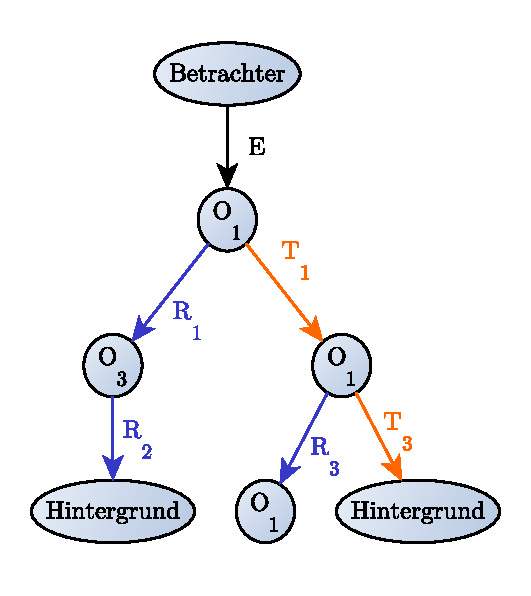
\includegraphics[width=0.5\textwidth]{img/ray_tracing_tree.pdf} \\
            Beispielszene &
            Gerichteter Strahlen-Baum \\
            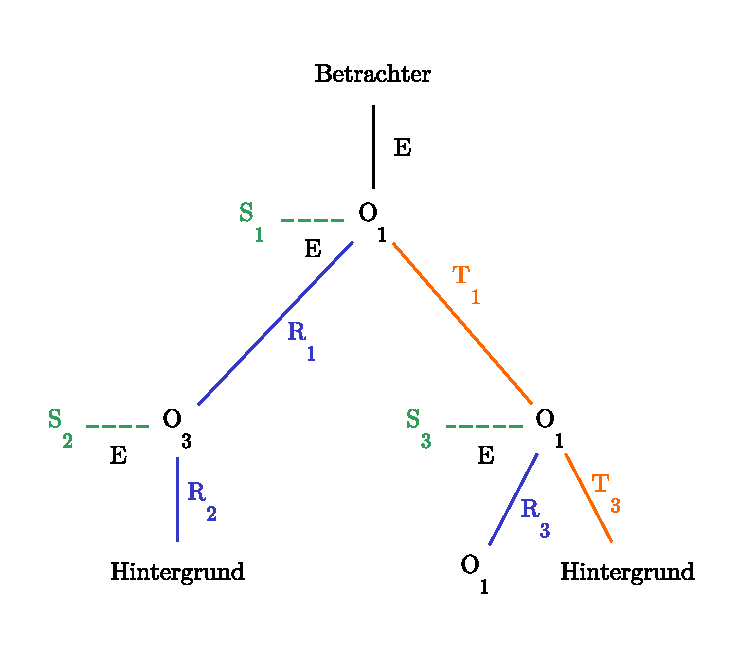
\includegraphics[width=0.5\textwidth]{img/ray_tracing_tree_schematic.pdf} \\
            Schematischer Strahlen-Baum
            nach~\citeauthor{glassner_introduction_1989}\protect\footnotemark{} \\
        \bottomrule
    \end{tabular}
\end{table}
\footnotetext{\cite[S.  17]{glassner_introduction_1989}}

\begin{minipage}{\linewidth}
\begin{lstlisting}[language=Python,caption={Eine abstrakte Umsetzung des
        Ray Tracings \protect\footnotemark.},
    label={fig:ray_tracing:high_level},captionpos=b,emph={ray_trace}]

def ray_trace(current_point, direction):
"""Traces light rays from current point in space in given direction.

:param current_point: current point in space
:type  current_point: three dimensional point object
:param direction:     the direction to trace
:type  direction:     three dimensional vector

:return:              the color for the given point
:rtype:               float
"""

    # Set color to currently set background color
    color = self.background_color

    # "pixels" is a list of all pixels of the image plane
    for pixel in pixels:

        # Returns the ray passing through the given
        # pixel from the eye
        ray = ray_at_pixel(pixel)

        # object_list is a list containing all the meshes contained in
        # the scene to render
        for object in object_list:
            p = intersect(ray, object)

            if object.is_reflective:
                reflection_vector = reflect(direction, object)
                reflected_color   = ray_trace(p, reflection_vector)
                color = color + object.coeff * reflected_color
            # end if

            if object.is_refractive:
                refracted_vector = refract(direction, object)
                refracted_color  = ray_trace(p, refracted_vector)
                color = color + object.coeff * refracted_color
            # end if

            for light in incoming_lights_at(p):
                if not is_shadow_ray(p, light.position):
                    color = color + calc_lighting(p, direction, light, object)
                # end if
            # end for lights
        # end for objects
    # end for pixels

    return color
# end def ray_trace
\end{lstlisting}
\footnotetext{Algorithmus in Pseudocode
    gemäss~\cite[Seite 283]{glassner_introduction_1989}}
\end{minipage}


